\documentclass[sigconf,nonacm]{acmart}
\settopmatter{printacmref=false,printfolios=true}
\renewcommand\footnotetextcopyrightpermission[1]{}
\acmConference[COL764]{COL764: Information Retrieval and Web Search}{November 2026}{IIT Delhi}
\usepackage{amsmath,booktabs}
\setlength{\emergencystretch}{2em}
\graphicspath{{figures/}}
\newcommand{\sigmoid}{\operatorname{sigmoid}}
\newcommand{\logit}{\operatorname{logit}}
\title[SAFE-Judge]{SAFE-Judge: Shared Adaptive Feedback for Escalation in Relevance Assessment}
\author{Ayush Ahuja}
\affiliation{\institution{Indian Institute of Technology Delhi}\city{New Delhi}\country{India}}
\authornote{Entry number: 2023CS50911. COL764 final project report, 17 November 2026.}
\renewcommand{\shortauthors}{Ayush Ahuja}
\begin{document}
\begin{abstract}
An LLM's confidence can conceal systematic relevance errors that differ by query
and predicted class. We study whether a fixed human-label budget is better spent
using shared and query-local feedback about those errors. SAFE-Judge (Shared Adaptive Feedback for Escalation) maintains a
small table of error estimates, shrinks sparse local evidence toward shared
evidence, and repeatedly reviews the pair with the highest estimated query-weighted
error. It keeps unreviewed assessor labels unchanged. On TREC DL 2020, at 50\%
human review, query-average remaining automatic error is 0.539\%, compared with
1.086\% for global raw LARA. On 40 reserved TREC-COVID topics, the corresponding
means are 4.458\% and 5.250\%; the conditional query-bootstrap interval includes
zero. Query-local feedback improves over shared-only and shuffled-query controls.
The ranking of 59 official DL 2020 runs is preserved with Kendall's
$\tau_b=.9882$. Comparisons with separate class thresholds, paid target
calibration and classical/neural baselines examine when feedback improves
review allocation under a matched human-label budget.
\end{abstract}
\keywords{relevance assessment, selective prediction, human review, query-local calibration}
\maketitle

\section{Introduction}
Relevance judgments make IR experiments reusable, but acquiring them is costly.
Compact LLMs offer cheap preliminary labels; their mistakes make selective human
review essential. LARA already learns an online calibration model, allocates
human judgments and debiases the remaining labels~\cite{lara}. The question here
is narrower: \emph{does feedback attached to a query improve the allocation of a
fixed review budget beyond global confidence calibration?}

Our pilot on DL 2019 accepted 50.02\% of pairs at confidence 0.90, with 9.78\%
observed selective error. Yet confidence concealed class asymmetry and query
variation. The nine highest-error-rate queries contained 34.4\% of all errors
but only 17.0\% of pairs. A corresponding descriptive check on DL 2020 finds
56.7\% of errors in eleven queries containing 27.1\% of pairs
(Figure~\ref{fig:queries}). These observations motivate local feedback; they do
not by themselves show that the errors are predictable before review.

Our hypothesis is that shared and local feedback reduce query-average label
error compared with confidence review and LARA at equal human-label cost.
The contributions are an explicit budgeted policy, component
controls testing its query structure, and an evaluation that separates label
error, class coverage and retrieval-system fidelity. We also report unsuccessful
threshold and calibration alternatives. DL 2019 is discovery data; DL 2020 and
biomedical COVID provide subsequent evaluations with frozen policy settings.
All are previously inspected public benchmarks, so the evidence is exploratory.

\begin{figure*}[t]
\centering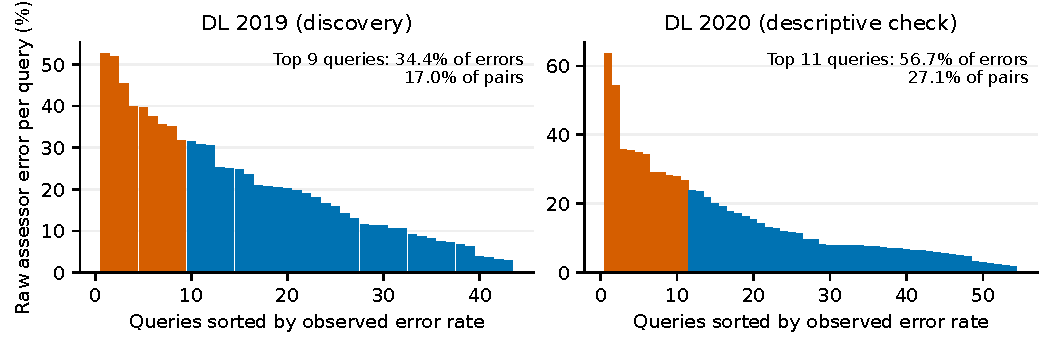
\includegraphics[width=\textwidth]{query_errors.pdf}
\caption{Errors differ across queries. Bars show raw binary error rates, sorted
using evaluation gold for diagnosis only. Orange marks the highest-error 20\%
of queries, rounded up. Query size and relevance prevalence also vary; the plot
does not identify a causal source of model error.}\label{fig:queries}
\Description{Sorted raw assessor error rates for DL 2019 and DL 2020, with error and pair shares of the highest-error queries.}
\end{figure*}

\section{Related Work}
LARA~\cite{lara} directly addresses acquisition. In the pinned binary code,
topic grouping reserves review quotas per query but retains one shared
calibrator. Grouping alone is therefore not our novelty claim.
We estimate errors of unchanged labels from shared and local
observations, whereas LARA calibrates relevance probabilities and debiases
automatic labels. Budgeted assessment and selection for comparing systems also
predate LLMs~\cite{carterette}.

Oosterhuis et al.~\cite{oosterhuis} use prediction-powered inference (PPI) and
conformal risk control (CRC) for retrieval-metric intervals. This includes
query-sensitive uncertainty, a different target from automatic-label coverage.
Our released-code comparison favors PPI on aggregate metric error. DIRAS
trains calibrated annotators~\cite{diras}; we allocate review around a frozen
assessor. Temperature scaling~\cite{guo} and CRC~\cite{crc} motivate controls,
but do not certify our adaptive error estimates. Shrinkage and class
stratification are established ingredients; our contribution is empirical.

\section{SAFE-Judge}
\subsection{Task and accounting}
For query $q$, let $D_q$ be its judged pool and $n_q=|D_q|$; the total pool has
$N=\sum_q n_q$ pairs. The assessor supplies relevance probability $p_i$, label
$a_i=\mathbf{1}[p_i\ge .5]$ and confidence $c_i=\max(p_i,1-p_i)$. A human purchase
reveals gold label $y_i$ and replaces that pair's label. Let $A$ be the remaining
automatic pairs and $H=N-|A|$ the paid review budget. Our objective is the
\emph{query-average automatic error} $E_Q$:
\begin{equation}
 E_Q=\frac{1}{|Q|}\sum_{q\in Q}\frac{1}{n_q}
       \sum_{i\in A\cap D_q}\mathbf{1}[a_i\ne y_i].
 \label{eq:loss}
\end{equation}
We also report \emph{pooled automatic error}
$E_P=\sum_{i\in A}\mathbf{1}[a_i\ne y_i]/N$ and \emph{selective error}
$R=\sum_{i\in A}\mathbf{1}[a_i\ne y_i]/|A|$. $E_Q$ averages errors per query;
$E_P$ divides mistakes by all pairs, and $R$ divides by automatic pairs only.
Equal-query and pooled error differ when query sizes vary.
All sentinels, calibration and review
labels count once. Human responses are simulated with existing judgments and
assumed exact; these are label counts, not measured annotation times.

\subsection{Error estimates and acquisition}
We form six bins $b$: predicted No/Yes crossed with confidence intervals
$[.5,.8)$, $[.8,.95)$ and $[.95,1]$. Initialize each pair's error prior
$e_i^0=\operatorname{clip}(1-c_i,.01,.49)$, and let $m_b$ be its bin mean.
Among purchased labels, $n_{qb}$ counts observations and $z_{qb}$ counts errors
of the original assessor. Write $n_b=\sum_q n_{qb}$ and $z_b=\sum_q z_{qb}$.
Shared evidence excludes the current query:
\begin{align}
 \mu_{qb}&=\frac{10m_b+z_b-z_{qb}}{10+n_b-n_{qb}},\label{eq:shared}\\
 r_{qb}&=\frac{5\mu_{qb}+z_{qb}}{5+n_{qb}}.\label{eq:local}
\end{align}
Exclusion avoids counting the same local observations twice. Shrinkage keeps
sparsely reviewed cells close to shared evidence. A bin-specific log-odds offset
preserves the pair's original confidence ordering inside its cell:
\begin{equation}
 \widehat e_i=\sigmoid\!\left(\logit(e_i^0)+
               \logit(r_{q_i b_i})-\logit(m_{b_i})\right).
 \label{eq:error}
\end{equation}
Probabilities entering logits are clipped away from zero and one. Review the
unreviewed pair maximizing $\widehat e_i/n_{q_i}$, observe its label and update
the counts. The denominator aligns acquisition with Eq.~\eqref{eq:loss}.
Seeded ordering resolves ties.

Before adaptive review, sample one sentinel from each available query/predicted
class, preferring confidence at least .90. Sentinels consume the budget and stay
human-labelled; a budget shorter than the sentinel list buys a randomized prefix.
The chosen policy has no automatic label repair, local gating, forced periodic
exploration or information bonus. It was selected during earlier discovery and
then frozen with shared/local strengths 10/5.

For intuition, two equally confident cells can share prior error .10. With five
local observations, zero versus three errors gives $(.5+0)/10=.05$ versus
$(.5+3)/10=.35$, redirecting review toward the latter. These working estimates
are not certified posteriors: adaptive observations need not represent a cell.

\section{Experimental Setup}
DL 2019 has 9,260 judged pairs over 43 queries; DL 2020 has 11,386 over 54
queries~\cite{trec19,trec20}. Grades 2--3 are relevant. The COVID sample contains
100 uniformly sampled judged title/abstract pairs on each of 50 topics;
grades 1--2 are relevant~\cite{treccovid}. Ten development topics are reserved;
the primary label-risk evaluation uses the other 40 (4,000 pairs). Full-50-topic
results are secondary and overlap this cohort. The same frozen Qwen3.5-4B
revision~\cite{qwen} supplies canonical Yes/No token probabilities, with NF4
loading, FP16 computation and a 512-token total input limit. Prompts state the
collection's relevance definition. Consequently, transfer changes domain,
document form and rubric; it is not an isolated domain intervention.

Policies start fresh at 0, 10, 25, 50, 75 and 90\% review. DL 2020 and COVID use
seeds 6000--6009. Discovery results use their recorded earlier seed block.
We retain all four LARA adaptations: global (G) or per-topic (Q) acquisition,
each with raw or authors' normalized probability preprocessing. Reference parity
was checked against pinned binary LARA code. This changes the paper's original
assessor and datasets, so it is a same-score adaptation, not reproduction of its
published table values. Raw confidence and random review are controls. A common
33-topic DL 2019 pool additionally compares lexical active learning and a pinned
MiniLM cross-encoder~\cite{minilm}, charging temperature-calibration labels.

\begin{table*}[t]
\centering\small
\caption{At 50\% human review, lower is better; best means are bold.
All values are percentages.
DL19 is discovery. COVID uses the 40 reserved topics. $E_Q$ divides each query's
remaining mistakes by all its pairs; $R$ divides pooled mistakes by automatic
pairs. G/Q denote global/topic LARA. Every budget includes online calibration.}
\label{tab:main}\begin{tabular}{@{}lrrrrr@{}}
\toprule
Method & DL19 $E_Q$ & DL20 $E_Q$ & COVID $E_Q$ & DL20 $R$ & COVID $R$ \\
\midrule
\textbf{SAFE-Judge} & \textbf{2.128} & \textbf{0.539} & \textbf{4.458} & \textbf{1.333} & \textbf{8.915} \\
LARA G/raw & 4.452 & 1.086 & 5.250 & 2.758 & 10.500 \\
LARA G/norm & 5.055 & 1.825 & 5.425 & 4.356 & 10.850 \\
LARA Q/raw & 4.460 & 3.612 & 5.623 & 9.989 & 11.245 \\
LARA Q/norm & 4.748 & 4.474 & 5.945 & 12.154 & 11.890 \\
Confidence & 4.782 & 2.590 & 5.303 & 6.204 & 10.605 \\
Random & -- & 7.630 & 10.950 & 17.142 & 21.900 \\
\bottomrule
\end{tabular}

\end{table*}

\begin{figure*}[t]
\centering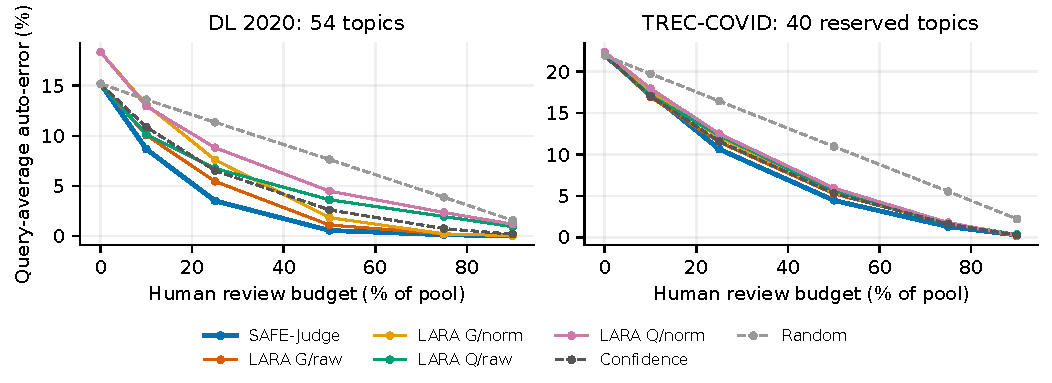
\includegraphics[width=\textwidth]{budget_error.pdf}
\caption{Remaining query-average automatic error versus total paid review.
Points are mean outcomes of separately initialized allocations; lines connect
measured budgets. This is a budget curve, not a certified risk bound.
All four LARA variants and both controls are retained.}\label{fig:budgets}
\Description{Budget-error curves on DL 2020 and the 40 reserved COVID topics for SAFE-Judge, four LARA variants, confidence and random review.}
\end{figure*}

Scoring took 33.12/45.19/32.46 minutes on one Tesla T4 for DL 2019/DL 2020/COVID;
review policies make no additional LLM calls.
We report macro-F1, binary $\kappa$, Brier, ten-bin ECE, class-conditional
reliability, risk--coverage/AURC, class/query tails, label costs and inference
time. Mixed-label F1/$\kappa$ include human corrections; we do not assign
fabricated calibrated probabilities to corrected labels. Ranking evaluation
retains all 59 official DL 2020 passage runs and original top-ten positions,
using binary nDCG@10. Of 31,860 positions, 1,315 are unjudged and receive zero
gain under both reference and mixed qrels. COVID's sampled pool cannot support
official-run ranking evaluation.

Conditional 95\% paired query-bootstrap intervals use 20,000 resamples for
error and 2,000 for ranking, averaging seeds within queries. Ranking scores
and correlations are recomputed; fitting and acquisitions remain fixed.
Method-search uncertainty and multiplicity are unadjusted. Deterministic LARA
repetitions add no independent observations.

\begin{table}[t]
\centering\small
\caption{DL 2020 ranking fidelity at 50\% review, over all 59 official runs.
Higher $\tau_b$ is better; lower binary nDCG@10 MAE and maximum rank drop are
better. Drop is the mean of each allocation's largest downward rank change.}
\label{tab:ranking}\begin{tabular}{@{}lrrr@{}}
\toprule
Method & $\tau_b$ & MAE & Drop \\
\midrule
SAFE-Judge & \textbf{0.9882} & 0.0113 & \textbf{2.8} \\
LARA G/raw & 0.9871 & \textbf{0.0030} & 3.0 \\
LARA G/norm & 0.9649 & 0.0234 & 3.0 \\
LARA Q/raw & 0.9703 & 0.0310 & 3.0 \\
LARA Q/norm & 0.9681 & 0.0501 & 3.0 \\
Confidence & 0.9607 & 0.0383 & 4.0 \\
Random & 0.9409 & 0.0195 & 5.9 \\
\bottomrule
\end{tabular}

\end{table}

\begin{table}[t]
\centering\small
\caption{Separate DL 2019 common-cohort comparison: 7,328 pairs, 33 topics,
3,664 total human labels, and three allocation seeds. T denotes temperature
scaling. $E_P$ and $R$ are error rates; $\gamma$ is automatic coverage.
MiniLM pays 1,932 external calibration labels within the total budget.}
\label{tab:classical}\begin{tabular}{@{}lrrrr@{}}
\toprule
Method & $E_P$ \% & $R$ \% & $\gamma$ \% & F1 \\
\midrule
Lexical AL & 9.548 & 19.096 & 50.00 & 0.8632 \\
MiniLM + T & 15.993 & 20.944 & 76.36 & 0.8114 \\
LARA G/norm & 4.326 & 8.652 & 50.00 & 0.9447 \\
SAFE-Judge & \textbf{2.543} & \textbf{5.086} & 50.00 & \textbf{0.9674} \\
\bottomrule
\end{tabular}

\end{table}

\section{Results}
\subsection{Label quality and domain shift}
At half review, SAFE-Judge reduces DL 2020 query-average error from
global raw LARA's 1.086\% to 0.539\% (Table~\ref{tab:main}). Pooled error is
0.667\% versus 1.379\%, corresponding to 75.9 versus 157 remaining mistakes on
average. The SAFE-Judge-minus-LARA query difference is $-0.547$ percentage points
(pp), with conditional 95\% interval $[-1.119,-0.095]$. SAFE-Judge beats all four
tested LARA means at this budget. Shared-only updating gives 1.270\% query error;
removing query-size weighting gives 0.540\%, suggesting that the local update
is the more consequential component on this pool.

On the 40 reserved COVID topics, SAFE-Judge has 4.458\% total error and
8.915\% selective risk; global raw LARA has 5.250\% and 10.500\%, respectively.
The query difference is $-0.793$ pp, with interval $[-1.748,+0.053]$; the
mean advantage is uncertain. Across all 50 topics, SAFE-Judge gives 3.950\%
versus 5.060\% total error (difference interval $[-1.936,-0.364]$ pp).
This cohort includes development topics and overlaps the primary cohort;
it is not independent confirmation. At 90\% review on reserved topics,
global raw LARA can outperform SAFE-Judge. Transfer evidence supports a mean
gain at half review, not superiority at every budget or domain.

\subsection{Class coverage and mechanism}
The DL 2020 gain has a material cost: only 0.30\% of the assessor's positive
predictions remain automatic. Two of ten SAFE-Judge allocations accept no positive
labels. Global raw LARA accepts no final positives in every run. Empty-class
risk is undefined, not zero. On COVID, SAFE-Judge retains 29.93\% of original
positives, with mean worst-class risk 10.19\%, compared with global raw LARA's
14.08\%. Thus class coverage changes the interpretation of the web and
biomedical results.

Discovery controls hold query-size weighting off and compare real versus
shuffled groups. At half review, SAFE-Judge error is 2.469\% with real queries and
4.696\% with shuffled groups; shared-only gives 4.348\% and 4.353\%.
The real-versus-shuffled contrast interval is approximately $[-4.00,-0.83]$ pp. This supports
informative grouping beyond extra parameters, while grouping also changes
sentinels and therefore does not isolate updating alone.

\subsection{Separate thresholds and target calibration}
Separate No/Yes confidence cutoffs are selected from 200 paid labels on disjoint
queries, minimizing estimated worst-class risk with 5\% automatic coverage in
each raw class. DL 2020 worst-class risk falls from confidence review's 40.32\%
to 38.08\%, but exceeds normalized global LARA's 34.06\%. A gold-only diagnostic
reaches 23.67\%, suggesting confident positive errors constrain this prefix
family; this does not rule out other policies. On COVID, thresholds give 13.86\%
versus confidence review's 14.88\% and SAFE-Judge's 10.19\%.

At 2,500 total COVID labels, free SAFE-Judge allocation gives 3.950\% error.
Reserving 200 development labels gives 4.464\%; adding Platt scaling gives
4.542\%. Reserving 1,000 labels gives 5.570\% without scaling and 5.690\% with
scaling. These settings do not repay their cost on this pool; cheaper or
amortized calibration remains possible.

\subsection{Retrieval-system fidelity}
LARA evaluates system ordering using Kendall's $\tau$ and maximum rank drop,
with MAP for binary relevance and nDCG for graded relevance~\cite{lara}.
Our ranking target is binary nDCG@10. Table~\ref{tab:ranking} compares all seven
policies on the same 59 DL 2020 systems and review budget. SAFE-Judge gives
$\tau_b=.9882$ and mean maximum drop 2.8, versus .9871 and 3.0 for global raw
LARA. Its Spearman correlation is .9992. LARA has lower nDCG@10 MAE
(.00299 versus .01128), while the conditional interval for the $\tau_b$
difference is $[-.0136,.0200]$. Lower label error therefore does not establish
better metric estimation or significantly better ordering. Full automation
already gives $\tau_b=.9147$, so simply exceeding .90 is a weak criterion here.

\subsection{Classical and neural assessor baselines}
Table~\ref{tab:classical} uses a separate common DL 2019 cohort to compare
lexical active learning, temperature-scaled MiniLM, LARA and SAFE-Judge.
SAFE-Judge has 2.543\% pooled auto-error and .9674 mixed-label macro-F1;
normalized global LARA gives 4.326\% and .9447. MiniLM's calibration cost leaves
76.36\% of evaluation pairs automatic, compared with 50\% for the other methods.
These differences include assessor choice and calibration overhead, and are
distinct from the same-Qwen allocation comparisons in Table~\ref{tab:main}.

\section{Limitations and Conclusion}
The frozen binary assessor was not adapter-trained; fixed binary-to-grade
ranking mappings do not make it a graded assessor. Public-benchmark
contamination is possible. Topics were previously inspected, and auxiliary
public data informed discovery. COVID truncates 1,393/5,000 inputs; longer
context, prompt paraphrases, genuine self-consistency and fresh blind audits
remain untested. Qrel incompleteness and exact-human simulation limit practical
interpretation. Independent audits fall back to full human review on every
tested DL 2020 run, so allocation gains lack an economical release certificate.

Within these limits, SAFE-Judge improves budget allocation on DL 2020
and yields a promising mean transfer result on COVID. Class coverage and score
fidelity remain separate objectives. The supplement records the complete binary
metrics, substantive failed approaches, graded diagnostics, 50 manually reviewed
failures, efficiency, statistical procedures and reproducibility requirements.

\paragraph{Artifacts and AI use.}
Code, settings, scores and ledgers:
\url{https://github.com/Ayush-Ahuja/SAFE-Judge}.
The research motivation, interpretation and final experimental decisions are
ours. We ran GPU inference and manually reviewed 50 failures. ChatGPT/Codex
assisted with literature review, mathematical formulations, code, CPU analyses
and drafting. We take responsibility for all claims. Full AI disclosure
accompanies the code.

\bibliographystyle{ACM-Reference-Format}
\bibliography{references}
\end{document}
